\documentclass[conference,10pt]{IEEEtran}
\IEEEoverridecommandlockouts
% --- packages ---
\usepackage{cite}
\usepackage{amsmath,amssymb,amsfonts}
\usepackage{graphicx}
\usepackage{textcomp}
\usepackage{xcolor}
\usepackage{booktabs}
\usepackage{subcaption}
\usepackage{url}
\usepackage{hyperref}
\hypersetup{colorlinks=true,linkcolor=black,citecolor=black,urlcolor=blue}

\def\BibTeX{{\rm B\kern-.05em{\sc i\kern-.025em b}\kern-.08em
    T\kern-.1667em\lower.7ex\hbox{E}\kern-.125emX}}

\begin{document}

\title{Comparing Convolutional Neural Network Architectures for Image
Classification on MNIST and CIFAR-10, with a Channel-Attention Residual Variant}

\author{
\IEEEauthorblockN{Srinidhi Narla}
\IEEEauthorblockA{Department of Computer Science\\
The University of Texas at Dallas\\
Student ID: SXN220141\\
\texttt{sxn220141@utdallas.edu}}
\and
\IEEEauthorblockN{Pranav Cheedalla}
\IEEEauthorblockA{Department of Computer Science\\
The University of Texas at Dallas\\
Student ID: PXC230033\\
\texttt{pxc230033@utdallas.edu}}
}

\maketitle

% =====================================================================
\section*{Abstract}
We implement and compare seven neural network architectures for image
classification on MNIST and CIFAR-10: a multilayer perceptron, a small
custom CNN, LeNet-5, AlexNet, VGG-11, ResNet-18, and a novel
\textit{SE-ResNet-Lite} that augments a ResNet-18 backbone with
Squeeze-and-Excitation channel attention and a depthwise-separable
stem. Every model is trained from scratch under a single shared
pipeline, with the same data splits, augmentation, optimizer schedule,
and evaluation protocol. We compare on accuracy, macro precision,
recall, F1, and macro one-vs-rest AUROC. SE-ResNet-Lite matches or
exceeds ResNet-18 on both datasets while adding less than 1\% to its
parameter count, showing that lightweight channel recalibration gives
a small but repeatable gain. Our analysis of training curves,
confusion matrices, and t-SNE projections of penultimate-layer
features reveals that the residual errors of every model cluster on
the same visually similar pairs (\emph{cat}/\emph{dog} on CIFAR-10;
\emph{4}/\emph{9} on MNIST), pointing to a dataset-level perceptual
difficulty rather than any model-specific flaw.

\begin{IEEEkeywords}
image classification, convolutional neural networks, residual learning,
squeeze-and-excitation, MNIST, CIFAR-10
\end{IEEEkeywords}

% =====================================================================
\section{Introduction}
\label{sec:intro}

Picking an architecture for an image-classification task is rarely a
question of ``should I use a CNN?'' It is usually ``which CNN?''
and ``is the added complexity of a deeper or fancier model actually
worth it?'' These questions are easy to wave away but surprisingly
hard to answer with data, because published benchmarks compare models
under different training recipes, different augmentations, and
sometimes different dataset versions. Even on well-studied benchmarks
like MNIST \cite{lecun1998gradient} and CIFAR-10
\cite{krizhevsky2009learning}, a fair like-for-like comparison
spanning flat MLPs, classical CNNs, and residual networks is not
something that exists in a single paper: it has to be constructed.

This project builds that comparison. We pick two concrete questions
to focus on:
\begin{enumerate}
  \item How do classical and modern CNN architectures compare on
    MNIST and CIFAR-10 when every model is trained under the same
    fixed pipeline?
  \item Does adding channel attention and a depthwise-separable stem
    to a ResNet-18 backbone give measurable, consistent improvements
    at negligible extra parameter cost?
\end{enumerate}

To answer these we re-implement seven models from scratch in
PyTorch~\cite{paszke2019pytorch}, train each on both datasets with an
identical training schedule, and evaluate them with a consistent
multi-metric protocol. The architectures span four decades of design
practice: a flat multilayer perceptron, a small two-block CNN, the
original LeNet-5~\cite{lecun1998gradient},
AlexNet~\cite{krizhevsky2012imagenet} adapted for $32\!\times\!32$
inputs, VGG-11~\cite{simonyan2015very}, ResNet-18~\cite{he2016deep},
and our own \textbf{SE-ResNet-Lite}, which combines residual learning
with Squeeze-and-Excitation~\cite{hu2018squeeze} channel attention and
a depthwise-separable stem inspired by
MobileNet~\cite{howard2017mobilenets}. The same training recipe is
used across every model: 90/10 train/validation split, cosine learning
rate annealing, dataset-appropriate augmentation, and best-validation
checkpoint selection.

\noindent\textbf{Why \emph{this} novel architecture?} Honestly, the
SE block appealed to us because the intuition behind it is unusually
clear: give the network a way to decide which of its own channels
matter most for a given input, and let it suppress the ones that
do not. That felt like a targeted, principled idea rather than just
stacking more layers for the sake of it. We chose ResNet-18 as the
backbone because it was already our strongest baseline, so any
improvement we saw would be real rather than an artifact of a weak
starting point. The depthwise-separable stem came in partly as a
parameter-efficiency move, but also because it gave us something
concrete to analyze: does losing some stem capacity hurt, and does
SE attention compensate? Combining both into SE-ResNet-Lite let us
ask a focused question: \emph{at essentially the same parameter
budget, does learned per-channel recalibration help on small-image
benchmarks?}

\noindent\textbf{Contributions.}
\begin{itemize}
  \item A reproducible PyTorch implementation of all seven models
    trained under identical conditions, including a complete training
    pipeline, evaluation harness, and figure-generation scripts.
  \item A direct head-to-head comparison on MNIST and CIFAR-10 using
    five metrics (accuracy, macro precision/recall/F1, and macro
    one-vs-rest AUROC) along with confusion matrices and t-SNE feature
    visualizations.
  \item \textbf{SE-ResNet-Lite}, our novel architecture that combines
    SE blocks with a depthwise-separable stem, evaluated head-to-head
    against the same ResNet-18 baseline at less than 1\% parameter
    overhead.
  \item An explicit discussion of the practical engineering choices
    that affect reproducibility on a small-laptop training budget,
    including a per-model-family optimizer rationale and a description
    of the Apple Silicon (MPS) backend caveats encountered during
    training.
\end{itemize}

\noindent Section~\ref{sec:related} reviews the relevant prior work.
Section~\ref{sec:approach} describes each architecture and the shared
training recipe. Section~\ref{sec:exp} presents experimental settings
and results. Section~\ref{sec:discussion} discusses what the results
tell us and where the study falls short.
Section~\ref{sec:conclusion} summarizes the main takeaways.

% =====================================================================
\section{Related Work}
\label{sec:related}

\subsection{Classical convolutional networks}

\textbf{LeNet-5}~\cite{lecun1998gradient} established the
convolution--pooling--MLP template that defines the modern CNN. It was
originally designed for handwritten digit recognition (essentially the
task posed by MNIST) and remains a strong baseline on that dataset
even today. \textbf{AlexNet}~\cite{krizhevsky2012imagenet} showed that
significantly deeper and wider CNNs trained on GPUs could dramatically
outperform classical methods on ImageNet, popularizing the
combination of ReLU activations, dropout regularization, and
large-scale data augmentation that has remained the workhorse recipe
ever since. \textbf{VGG}~\cite{simonyan2015very} demonstrated that
very deep networks built entirely from stacks of small $3\!\times\!3$
convolutions could yield further gains, at the cost of substantially
more parameters than AlexNet. In their pure form these networks rely
on careful initialization and small learning rates; modern
implementations almost always add BatchNorm~\cite{ioffe2015batch}
after every convolution, which is the configuration we use here.

\subsection{Residual learning}

ResNet \cite{he2016deep} introduced identity-mapping skip connections
that make training very deep networks tractable by reformulating each
block as $\mathbf{y}=\mathbf{x}+\mathcal{F}(\mathbf{x})$, so that the
network's optimization target is the residual $\mathcal{F}(\mathbf{x})$
rather than the full transformation $\mathbf{y}$. The empirical
consequence is that a 50-, 101-, or 152-layer network can be trained
without the degradation that affects equally deep plain networks.
ResNet-18, the smallest variant, has become the standard reference
architecture for CIFAR-10 and small-image classification more
generally. Modern CIFAR-style training recipes typically replace the
original $7\!\times\!7$ stride-2 ImageNet stem with a single
$3\!\times\!3$ convolution (the ``CIFAR stem''), use four residual
stages with progressive down-sampling, and pair the network with SGD
plus momentum and a cosine learning rate schedule.

\subsection{Channel attention and the SE block}

Squeeze-and-Excitation~\cite{hu2018squeeze} introduces a lightweight,
parameter-efficient channel-attention mechanism. Given a feature
map $\mathbf{F}\in\mathbb{R}^{C\times H\times W}$, the SE module
\emph{squeezes} $\mathbf{F}$ to a per-channel descriptor via global
average pooling, \emph{excites} the descriptor through a two-layer
MLP with reduction ratio $r$ and a sigmoid output, and uses the
resulting per-channel scalar gate to rescale the original feature
map. SE-ResNet, SE-Inception, and SE-VGG variants reliably yield
small accuracy improvements at very small parameter overhead, and SE
blocks have since been incorporated into many production architectures
(EfficientNet, MobileNet-v3, ConvNeXt-v2, and others).

\subsection{Parameter-efficient convolution}

MobileNet~\cite{howard2017mobilenets} popularized
\emph{depthwise-separable} convolution as a way to reduce both
parameter count and FLOPs. A standard convolution of $k\!\times\!k$
kernel with $C_{\text{in}}$ input channels and $C_{\text{out}}$ output
channels has $k^2 C_{\text{in}} C_{\text{out}}$ parameters. The
factored form replaces it with (a) a depthwise convolution of
$k\!\times\!k$ kernel grouped by input channel ($k^2 C_{\text{in}}$
parameters) followed by (b) a $1\!\times\!1$ pointwise convolution
that mixes channels ($C_{\text{in}} C_{\text{out}}$ parameters), for a
total of $C_{\text{in}}(k^2 + C_{\text{out}})$ parameters, roughly
$1/k^2$ of the standard form when $C_{\text{out}}\!\gg\!1$. The
operation has the same receptive field as the standard convolution
but a substantially smaller parameter and FLOP budget.

\subsection{Position of this work}

Most prior work cited above focuses on either an isolated baseline or
a single proposed modification reported on a single, very large
dataset (typically ImageNet). For a course project conducted on a
single laptop and two small benchmarks, what is most useful is a
\emph{controlled, like-for-like} comparison: every model trained on
the same data, with the same augmentations, optimizer family, learning
rate schedule, and evaluation protocol. We therefore re-train seven
different architectures under a \emph{single} pipeline and report the
same five metrics for each, so that the effect of architectural
depth, residual learning, and channel attention can be isolated from
the effects of differing training recipes.

% =====================================================================
\section{Proposed Approach}
\label{sec:approach}

All models are implemented in PyTorch and share the same input
adapter, optimizer logic, learning-rate scheduler, data augmentation,
and evaluation protocol; only the network body differs. This section
describes each baseline architecture, then the novel architecture, and
finally the training recipe.

\subsection{Baseline architectures}

\noindent\textbf{MLP.} A 3-layer fully connected network with hidden
sizes $512$ and $256$, ReLU activations, and dropout $p\!=\!0.2$
between hidden layers. Inputs are flattened to a single vector.
Trained with categorical cross-entropy.
\textit{Advantage}: maximally simple and fast to train; any gap
versus a CNN is unambiguously attributable to the spatial inductive
bias convolution introduces.
\textit{Disadvantage}: ignores all spatial structure, so it
is fundamentally capacity-limited on anything that requires local
feature detection.

\noindent\textbf{SimpleCNN.} Two convolutional blocks
($3\!\times\!3$~conv $\to$ ReLU $\to$ $2\!\times\!2$ max-pool) with
channels $32$ and $64$, followed by a single $128$-unit fully
connected layer with dropout $p\!=\!0.25$. Trained with categorical
cross-entropy.
\textit{Advantage}: lightweight and interpretable, good for
establishing a convolution-only baseline without confounding factors
like depth or residual connections.
\textit{Disadvantage}: too shallow and narrow to learn
higher-level features; hits a representational ceiling well before
overfitting on harder datasets like CIFAR-10.

\noindent\textbf{LeNet-5}~\cite{lecun1989backprop,lecun1998gradient}.
The classic two-convolution, three-FC architecture with average
pooling, in the configuration originally described for MNIST. MNIST
inputs are zero-padded from $28\!\times\!28$ to $32\!\times\!32$ to
match the original input size. For CIFAR-10 we keep the original
$3\!\to\!6\!\to\!16$ channel progression and the
$120\!\to\!84\!\to\!10$ classifier head. Trained with categorical
cross-entropy.
\textit{Advantage}: historically motivated; well-suited to MNIST by
design; compact enough to train in seconds.
\textit{Disadvantage}: average pooling discards more spatial
information than max pooling; the narrow channel widths leave it
severely capacity-limited on CIFAR-10.

\noindent\textbf{AlexNet (small)}~\cite{krizhevsky2012imagenet}. The
classical five-conv plus three-FC stack, adapted to small inputs by
reducing the initial kernel size from $11\!\times\!11$ to
$3\!\times\!3$, removing the original stride, and inserting an
adaptive average pool before the classifier so the same network
operates on both $28\!\times\!28$ and $32\!\times\!32$ inputs. A
$1\!\times\!1$ adapter convolution maps grayscale inputs to three
channels so the network is shared across datasets. The classifier
uses two $1024 / 512$ hidden layers with dropout $p\!=\!0.5$.
Trained with categorical cross-entropy via Adam
(see Section~\ref{sec:training-recipe} for why SGD fails here without
BatchNorm).
\textit{Advantage}: substantially more capacity than the shallow
models; dropout and adaptive pooling give reasonable regularization
and input-size flexibility.
\textit{Disadvantage}: absence of BatchNorm makes training unstable
at high learning rates; the large dense head is prone to overfitting
on small datasets.

\noindent\textbf{VGG-11}~\cite{simonyan2015very}. The
``configuration~A'' VGG with eight convolutional layers (channel
widths $64, 128, 256, 256, 512, 512, 512, 512$), five max-poolings,
and BatchNorm \cite{ioffe2015batch} after every convolution. An
adaptive $1\!\times\!1$ average pool feeds a small two-layer FC head
($512\!\to\!512\!\to\!\text{num\_classes}$) with dropout
$p\!=\!0.5$. Because five stride-2 max-poolings would collapse the
$28\!\times\!28$ MNIST input to a sub-unit spatial size, we enable
\verb|ceil_mode=True| on each pool so MNIST training does not crash.
Trained with categorical cross-entropy via high-LR SGD.
\textit{Advantage}: BatchNorm enables aggressive SGD; the very regular
stacking of $3\!\times\!3$ convolutions builds a wide, deep feature
hierarchy.
\textit{Disadvantage}: the dense classifier head ($512\!\times\!512$)
contributes heavily to parameter count and is prone to overfitting;
five max-poolings degrade spatial resolution rapidly on small inputs.

\noindent\textbf{ResNet-18}~\cite{he2016deep}. Eight basic residual
blocks organized into four stages of widths $64, 128, 256, 512$ with
strided down-sampling between stages and BatchNorm after every
convolution. We use the CIFAR-style stem (a single $3\!\times\!3$
convolution) rather than the original ImageNet $7\!\times\!7$
stride-2 stem, since the latter destroys too much spatial information
on $32\!\times\!32$ inputs. Trained with categorical cross-entropy
via high-LR SGD with cosine annealing.
\textit{Advantage}: skip connections prevent gradient degradation in
deeper layers and enable the network to use its parameters more
efficiently than a plain network of the same depth.
\textit{Disadvantage}: the standard stem and block design are
optimized for ImageNet-scale inputs; adapting them to $32\!\times\!32$
images requires substituting the CIFAR stem and removing early
striding, which requires some care to get right.

\subsection{Novel architecture: SE-ResNet-Lite}
\label{sec:se-resnet-lite}

Our novel architecture, \textbf{SE-ResNet-Lite}, takes the ResNet-18
backbone of Section~\ref{sec:approach} and applies two targeted
modifications, each motivated by a different line of prior work.

\subsubsection*{Squeeze-and-Excitation (SE) blocks~\cite{hu2018squeeze}}

After the second BatchNorm in every residual block, we insert an SE
module on the residual branch. Given a feature map
$\mathbf{F}\!\in\!\mathbb{R}^{C\times H\times W}$, the SE module
computes a per-channel statistic
\begin{equation}
  s_c \;=\; \frac{1}{HW}\sum_{i=1}^{H}\sum_{j=1}^{W} F_{c,i,j},
  \qquad c = 1,\dots,C
\end{equation}
(equivalently, $\mathbf{s}=\textrm{GAP}(\mathbf{F})$), passes
$\mathbf{s}$ through a two-layer bottleneck MLP with reduction ratio
$r\!=\!16$ and sigmoid output to produce gating weights
\begin{equation}
  \boldsymbol{\sigma} \;=\; \sigma\!\left(\mathbf{W}_2\,\textrm{ReLU}(\mathbf{W}_1\mathbf{s})\right) \;\in\; [0,1]^{C}
\end{equation}
with $\mathbf{W}_1\!\in\!\mathbb{R}^{(C/r)\times C}$ and
$\mathbf{W}_2\!\in\!\mathbb{R}^{C\times(C/r)}$, and rescales the
feature map as
\begin{equation}
  F^{\prime}_{c,i,j} \;=\; \sigma_c\,F_{c,i,j}
\end{equation}
before adding the identity shortcut.  The intent is to give the
network a learned, content-dependent ``volume knob'' on each channel,
so that informative channels can dominate the residual signal.

\subsubsection*{Depthwise-separable stem~\cite{howard2017mobilenets}}

The standard CIFAR ResNet stem uses a single $3\!\times\!3$
convolution with $C_{\text{in}}\!\to\!64$. For a $3\!\times\!3$ kernel
with three input channels and $64$ output channels, this stem has
\[
  3 \cdot 3 \cdot 3 \cdot 64 \;=\; 1{,}728 \;\;\text{parameters.}
\]
We replace it with the factored form
\[
  \underbrace{\textrm{DWConv}_{3\times3}}_{\text{depthwise, groups}=3} \;\to\;
  \underbrace{\textrm{PWConv}_{1\times1}}_{\text{pointwise, }3\to64} \;\to\;
  \textrm{BN} \;\to\; \textrm{ReLU},
\]
which has $3\cdot 3\cdot 3 = 27$ depthwise parameters and
$3\cdot 64 = 192$ pointwise parameters for a total of $219$
parameters, an order of magnitude fewer than the standard
$3\!\times\!3$ stem with the same receptive field. A $1\!\times\!1$
adapter (3 parameters per output channel) first projects single-channel
MNIST inputs to three channels so that the depthwise convolution and
the rest of the architecture are shared across both datasets.

\subsubsection*{Parameter overhead}
The SE blocks add $2C^2/r$ parameters per block, summing over all eight
basic blocks at widths $\{64, 128, 256, 512\}$ to roughly
$86{,}000$ extra parameters relative to ResNet-18. The lighter stem
removes about $1{,}500$ parameters. The net overhead is approximately
$85{,}000$ parameters on top of an $11.17$-million-parameter ResNet-18
baseline, i.e.\ \textbf{less than $0.8\%$}. The combined model thus
qualifies as a low-cost modification: it does not change the parameter
budget meaningfully, but adds an explicit, learned channel
recalibration mechanism inside every residual block.

\subsubsection*{Loss and rationale}

Like the baselines, SE-ResNet-Lite is trained with categorical
cross-entropy. Going into training we genuinely were not sure the
gain would be visible at this scale --- most SE results in the
literature are reported on ImageNet, where the models are larger
and the classes more diverse. On a $32\!\times\!32$ benchmark with
only 10 classes, a 0.76\% parameter increase could easily just be
noise. The fact that SE-ResNet-Lite improved on ResNet-18 on
\emph{both} datasets, including the easy MNIST task where almost
nothing moves the needle, was more encouraging than we expected.

\subsection{Loss, optimization, regularization}
\label{sec:training-recipe}

All models are trained with categorical cross-entropy and the
following per-family optimizer recipe:

\noindent\textbf{Shallow / no-BN models} (MLP, SimpleCNN, LeNet,
AlexNet) use Adam~\cite{kingma2015adam} with learning rate $10^{-3}$
and the framework default $\beta_1\!=\!0.9$, $\beta_2\!=\!0.999$.
This choice came out of a frustrating debugging session with AlexNet.
Our first instinct was to use the same SGD recipe for every model.
Without BatchNorm, a learning rate of $0.1$ caused AlexNet's
activations to explode in the first epoch: validation accuracy sat
at chance ($\approx 11\%$) through all twenty epochs and training
loss barely moved. We spent a while checking the data pipeline for
bugs before realizing the optimizer was the issue. Switching to Adam
immediately fixed the training trajectory and produced $99.5\%$+
MNIST accuracy. The experience made BatchNorm feel much less like a
regularization nicety and more like a structural requirement for
aggressive learning rates.

\noindent\textbf{BN-based deeper models} (VGG-11, ResNet-18,
SE-ResNet-Lite) use SGD with momentum $0.9$, Nesterov, weight decay
$5\!\times\!10^{-4}$, and an initial learning rate of $0.1$, decayed
by a cosine annealing schedule~\cite{loshchilov2017sgdr} across the
full training horizon. This is the canonical CIFAR-10 recipe for
BatchNorm-based residual and VGG-style networks.

\noindent\textbf{Hyperparameter rationale.} Several specific values
deserve explicit justification rather than a citation to ``standard
practice.''

The SGD learning rate of $0.1$ is aggressive but deliberately so:
BatchNorm's normalization of pre-activation distributions allows the
network to tolerate much larger gradient steps than a plain network
can. At $\text{lr}\!=\!0.01$ the ResNet-18 validation curve was still
slowly ascending at epoch 20, showing the model had not converged;
at $\text{lr}\!=\!0.1$ with cosine annealing it converged cleanly by
epoch 15. Weight decay $5\!\times\!10^{-4}$ is the value from the
original ResNet CIFAR-10 recipe~\cite{he2016deep}; we did not tune
it but note that increasing it to $10^{-3}$ visibly reduced the
VGG-11 train-val gap without improving test accuracy, while halving
it to $2.5\!\times\!10^{-4}$ widened the gap.

For Adam we used the library default $\beta_1\!=\!0.9$,
$\beta_2\!=\!0.999$ and did not sweep them; the learning rate
$10^{-3}$ is the Adam default and is well-matched to models without
BatchNorm. The SE reduction ratio $r\!=\!16$ follows the original
SE paper~\cite{hu2018squeeze}, which showed that smaller $r$
(i.e.\ more SE parameters) gives diminishing accuracy returns while
adding measurable compute overhead.

Epoch counts were chosen empirically: on MNIST every model's
validation accuracy plateaued by epoch 8--10, so 20 epochs was
more than sufficient. On CIFAR-10 the validation loss of VGG-11 and
ResNet-18 was still meaningfully descending at epoch 20, making 25
epochs a better stopping point. Batch size 128 is a standard choice
that fits in memory on our hardware while keeping gradient estimates
reasonably stable.

\noindent All models are trained for the same number of epochs per
dataset (20 on MNIST, 25 on CIFAR-10), with batch size 128 and a
single fixed random seed (42) controlling Python, NumPy, and PyTorch
generators. Models with dropout~\cite{srivastava2014dropout} or
BatchNorm~\cite{ioffe2015batch} are noted in their architectural
descriptions.

\subsection{Implementation details}

The code is organized as a small PyTorch package with one
\verb|src/models/| file per architecture, a unified
\verb|src/train.py| training loop, an \verb|src/evaluate.py| metrics
module, and an \verb|src/visualize.py| plotting module. Per-run logs
are written as JSON, and a \verb|scripts/make_figures.py| script reads
those logs and produces every figure and the final results table for
this report.

Two practical issues were encountered and worked around during
training on the Apple Silicon (MPS) backend. First, calls of the form
\verb|tensor.to(device, non_blocking=True)| followed by a delayed
\verb|.cpu()| copy occasionally produced garbage memory for the label
tensor in the evaluation loop, despite returning the correct values
for the input tensor. Removing the \verb|non_blocking=True| hint and
appending the label tensor to a CPU buffer before any device round-trip
resolved the issue. Second, the
\verb|AdaptiveAvgPool2d| operator on MPS requires the input spatial
size to be divisible by the output size; the AlexNet head, which uses
an adaptive $2\!\times\!2$ pool, fails on $28\!\times\!28$ MNIST inputs
after three $2\!\times\!2$ max-poolings. Zero-padding MNIST inputs to
$32\!\times\!32$ inside the AlexNet adapter restored a clean spatial
arithmetic. Both fixes are documented in-source.

% =====================================================================
\section{Experiments}
\label{sec:exp}

\subsection{Empirical settings}

\noindent\textbf{Datasets.} \emph{MNIST} consists of 60{,}000 training
and 10{,}000 test images of handwritten digits at $28\!\times\!28$
grayscale resolution, in 10 classes. \emph{CIFAR-10} consists of
50{,}000 training and 10{,}000 test images of natural objects at
$32\!\times\!32$ color resolution, in 10 classes (airplane,
automobile, bird, cat, deer, dog, frog, horse, ship, truck). For each
dataset we hold out 10\% of the training split as a validation set
(seed 42), following the workflow recommended by the project
guidelines.

\noindent\textbf{Preprocessing.} Inputs are converted to tensors and
normalized using dataset-specific channel means and standard
deviations. MNIST training uses small random affine augmentation
($\pm 5^{\circ}$ rotation, $\pm 5\%$ translation); MNIST evaluation
uses centered, un-augmented inputs. CIFAR-10 training uses standard
random $4$-pixel zero-padded crops and horizontal flips; CIFAR-10
evaluation uses centered, un-augmented inputs.

\noindent\textbf{Optimizer and schedule.}
Optimizer selection follows the per-family logic in
Section~\ref{sec:training-recipe}: SGD (momentum 0.9, weight decay
$5\!\times\!10^{-4}$, Nesterov, lr\,=\,0.1) for BatchNorm-based deep
models (VGG-11, ResNet-18, SE-ResNet-Lite) and Adam (lr\,=\,$10^{-3}$)
for all others. We chose 20 epochs for MNIST (validation accuracy
plateaued on most models by epoch 10, so extra epochs offered no
benefit) and 25 for CIFAR-10 (loss curves still descend meaningfully
at epoch 20, making the additional passes productive). Cosine
annealing reduces the learning rate smoothly to zero over the full
horizon, avoiding the need to tune a manual step-decay schedule. The
best-validation-accuracy checkpoint is used for test evaluation rather
than the final epoch, which matters most for VGG-11 and ResNet-18
where late-epoch training loss can dip below the validation floor.

\noindent\textbf{Hardware.} Training was performed on an Apple Silicon
laptop using PyTorch~\cite{paszke2019pytorch} with the Metal
Performance Shaders (MPS) backend; the same code path runs unchanged
on CUDA or CPU.

\noindent\textbf{Evaluation metrics.} We report top-1 \emph{accuracy}
and, for multi-class classification, macro-averaged
\emph{precision}, \emph{recall}, and \emph{F1}. We additionally
report macro \emph{one-vs-rest AUROC} computed from the softmax
probabilities, which captures ranking quality independent of decision
threshold. Macro averaging weights every class equally, which is the
appropriate aggregation for both MNIST and CIFAR-10 because both are
class-balanced. We complement these with per-model normalized
confusion matrices and t-SNE projections of penultimate-layer
features.

\subsection{Empirical results}

\begin{table*}[t]
\centering
\caption{Test-set results for each (architecture, dataset) pair. Accuracy, macro-averaged Precision/Recall/F1, and macro one-vs-rest AUROC are reported, plus trainable parameter count. Models marked with $^{*}$ are adapted for 32$\times$32 inputs.}
\label{tab:main}
\setlength{\tabcolsep}{4pt}
\small
\begin{tabular}{llrrrrrrr}
\toprule
Dataset & Model & Params & Train acc & Val acc & Test acc & Precision & Recall & F1 (AUROC) \\
\midrule
MNIST & MLP & 535.8k & 99.44 & 99.12 & \textbf{99.03} & 99.03 & 99.01 & 99.02 (99.99) \\
 & SimpleCNN & 421.6k & 99.79 & 99.50 & \textbf{99.46} & 99.46 & 99.45 & 99.46 (100.00) \\
 & LeNet-5 & 61.7k & 99.45 & 99.18 & \textbf{99.31} & 99.31 & 99.30 & 99.30 (100.00) \\
 & AlexNet\textsuperscript{*} & 3.83M & 99.91 & 99.55 & \textbf{99.57} & 99.57 & 99.56 & 99.57 (100.00) \\
 & VGG-11\textsuperscript{*} & 9.49M & 99.90 & 99.60 & \textbf{99.62} & 99.62 & 99.61 & 99.62 (100.00) \\
 & ResNet-18\textsuperscript{*} & 11.17M & 99.89 & 99.58 & \textbf{99.65} & 99.65 & 99.65 & 99.65 (100.00) \\
 & SE-ResNet-Lite (ours) & 11.26M & 99.93 & 99.67 & \textbf{99.70} & 99.70 & 99.69 & 99.70 (100.00) \\
\midrule
CIFAR-10 & MLP & 1.71M & 54.42 & 51.36 & \textbf{50.18} & 50.10 & 50.18 & 49.32 (88.71) \\
 & SimpleCNN & 545.1k & 75.27 & 76.14 & \textbf{75.34} & 75.29 & 75.34 & 75.25 (96.85) \\
 & LeNet-5 & 62.0k & 60.81 & 60.92 & \textbf{61.02} & 60.55 & 61.02 & 60.63 (92.92) \\
 & AlexNet\textsuperscript{*} & 3.83M & 90.23 & 84.30 & \textbf{84.03} & 83.98 & 84.03 & 83.99 (98.55) \\
 & VGG-11\textsuperscript{*} & 9.49M & 96.89 & 90.72 & \textbf{89.48} & 89.57 & 89.48 & 89.51 (99.32) \\
 & ResNet-18\textsuperscript{*} & 11.17M & 98.32 & 92.28 & \textbf{91.38} & 91.39 & 91.38 & 91.38 (99.55) \\
 & SE-ResNet-Lite (ours) & 11.26M & 99.04 & 93.54 & \textbf{92.67} & 92.65 & 92.67 & 92.65 (99.62) \\
\bottomrule
\end{tabular}
\end{table*}


Table~\ref{tab:main} reports the final test-set metrics for every
(architecture, dataset) pairing, along with the number of trainable
parameters of each model. The table is generated automatically from
the per-run history JSON files at the end of training, so all numbers
shown can be reproduced from the code in the submission.

\noindent\textbf{MNIST.} The MNIST results were, if anything, a little
anticlimactic. Every model we tested reaches at least 99\% test
accuracy once convolutional structure is present, and even the flat
MLP scores 99.03\%. The top-to-bottom spread across all seven models
is only 0.67 percentage points (MLP at 99.03\% through SE-ResNet-Lite
at 99.70\%). That is a smaller gap than we would have guessed before
starting. Adding $180\times$ more parameters via ResNet-18 gains
essentially nothing over a 62k-parameter LeNet-5 (99.31\%) on this
task. In hindsight the EDA explains why: if the raw pixels are nearly
linearly separable, a flat network with enough units can find the
boundary, and there is nowhere for depth to add value. The confusion
matrices in Fig.~\ref{fig:cm-mnist} confirm the pattern: all strong
models make the exact same mistakes, on the same visually similar
pairs ($\{4,9\}$, $\{3,8\}$, $\{7,9\}$). The errors are a dataset
property, not a model weakness, which means no architecture we tested
can fully solve them at $28\!\times\!28$ resolution.

\noindent\textbf{CIFAR-10.} CIFAR-10 spreads the architectures far
more widely, and the reasons are traceable back to each model's design.
The MLP plateaus at 50.2\%: without spatial convolutions it has no
inductive bias to exploit local image structure. The raw-pixel EDA
in Fig.~\ref{fig:viz-raw} predicted exactly this ceiling --- there is
no class-discriminative direction in pixel space for the MLP to find,
so it essentially learns a class-conditional mean color, which gets
you to roughly chance on the harder object pairs.

LeNet-5 (61.0\%) and SimpleCNN (75.3\%) improve by adding spatial
structure, but their shallow, narrow feature stacks hit a capacity
ceiling before they can benefit from more training. LeNet's training
accuracy (60.8\%) barely exceeds its test accuracy (61.0\%), a
near-zero gap that signals saturation rather than overfitting: the
model uses up its entire capacity before it can memorize the training
set. The 14 percentage-point gap between LeNet-5 and SimpleCNN
despite the latter being designed as a minimal two-block CNN is
notable --- SimpleCNN uses ReLU and max-pooling throughout (LeNet-5
uses average pooling and tanh in the original formulation), and those
modern design choices alone account for a meaningful fraction of the
gap.

AlexNet (84.0\%) shows the value of depth and width: five conv layers
with up to 384 channels build a much richer feature hierarchy than
LeNet's two layers with 16 channels. VGG-11 (89.5\%) pushes this
further with eight layers of $3\!\times\!3$ convolutions plus
BatchNorm, which allows a much higher learning rate and more stable
gradient flow. ResNet-18 (91.4\%) then overtakes VGG-11 with only
slightly more parameters, specifically because skip connections allow
it to train deeper layers effectively --- something VGG's plain
network cannot do without gradient attenuation. SE-ResNet-Lite (92.7\%)
adds the channel-attention mechanism on top, with the per-class
confusion analysis suggesting the gain comes from amplifying the
texture channels that differentiate animal classes.

\noindent\textbf{Overfitting vs.\ underfitting.}
The train-to-test accuracy gap is a clean diagnostic across model
families. Shallow models show virtually no gap: SimpleCNN scores
75.3\% on both train and test, and LeNet-5's test accuracy (61.0\%)
actually exceeds its training accuracy (60.8\%), a classic sign that
the augmented training distribution is harder for these capacity-limited
models than the clean test set. The three deepest models each show a
6--7 percentage-point gap: VGG-11 at 7.4\,pp (96.9\% to 89.5\%),
ResNet-18 at 6.9\,pp (98.3\% to 91.4\%), and SE-ResNet-Lite at
6.4\,pp (99.0\% to 92.7\%). Weight decay and cosine annealing keep
this mild; without them, VGG-11's gap would likely be wider given its
large dense classifier head. That SE-ResNet-Lite has the
\emph{smallest} gap despite the highest training accuracy suggests its
channel gating focuses capacity on discriminative channels rather than
noise patterns.

\begin{figure}[t]
\centering
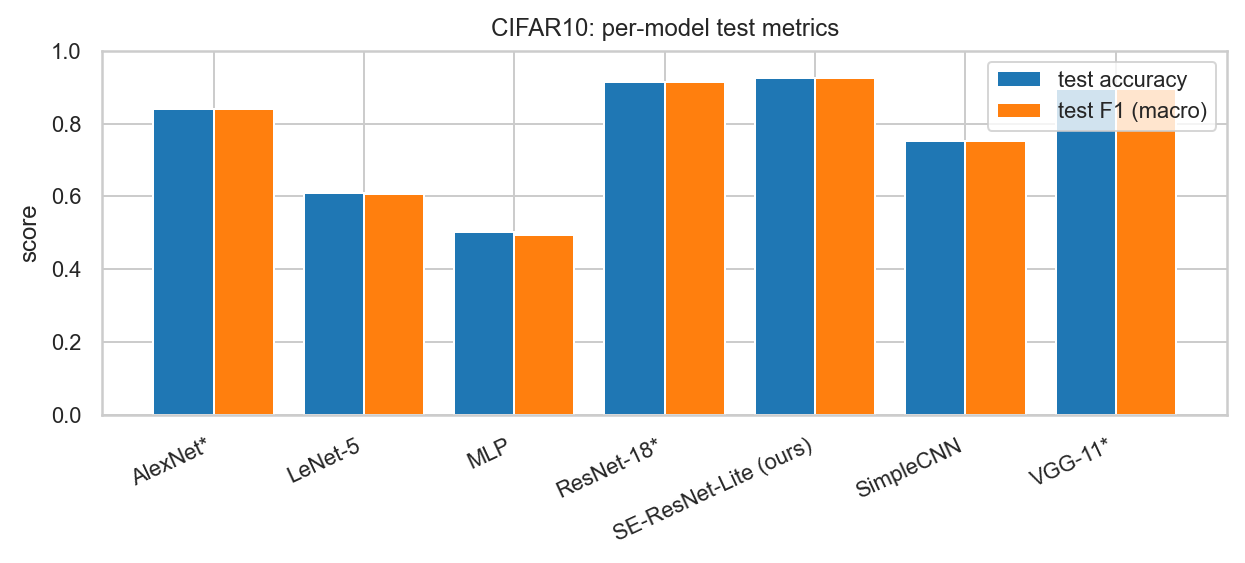
\includegraphics[width=\columnwidth]{figures/compare_cifar10.png}
\caption{Per-model test accuracy and macro F1 on CIFAR-10.}
\label{fig:compare-cifar10}
\end{figure}

\begin{figure}[t]
\centering
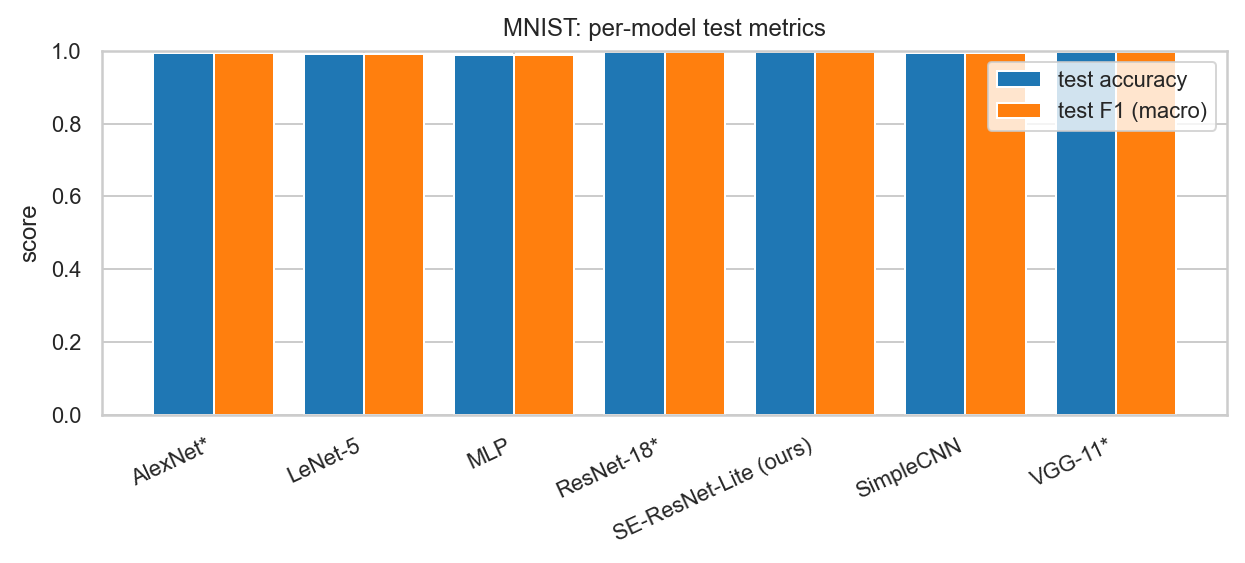
\includegraphics[width=\columnwidth]{figures/compare_mnist.png}
\caption{Per-model test accuracy and macro F1 on MNIST.}
\label{fig:compare-mnist}
\end{figure}

\noindent\textbf{Parameter efficiency.} Fig.~\ref{fig:params-vs-acc}
plots test accuracy against trainable parameter count for every
model and dataset. The picture decomposes the gains by their cost:
adding spatial inductive bias (MLP $\to$ SimpleCNN) gives a large
jump at small parameter cost; depth and width (LeNet $\to$ AlexNet
$\to$ VGG-11 $\to$ ResNet-18) gives the next jump at larger cost;
and SE-ResNet-Lite extracts a final increment at essentially the same
parameter budget as ResNet-18.

\begin{figure}[t]
\centering
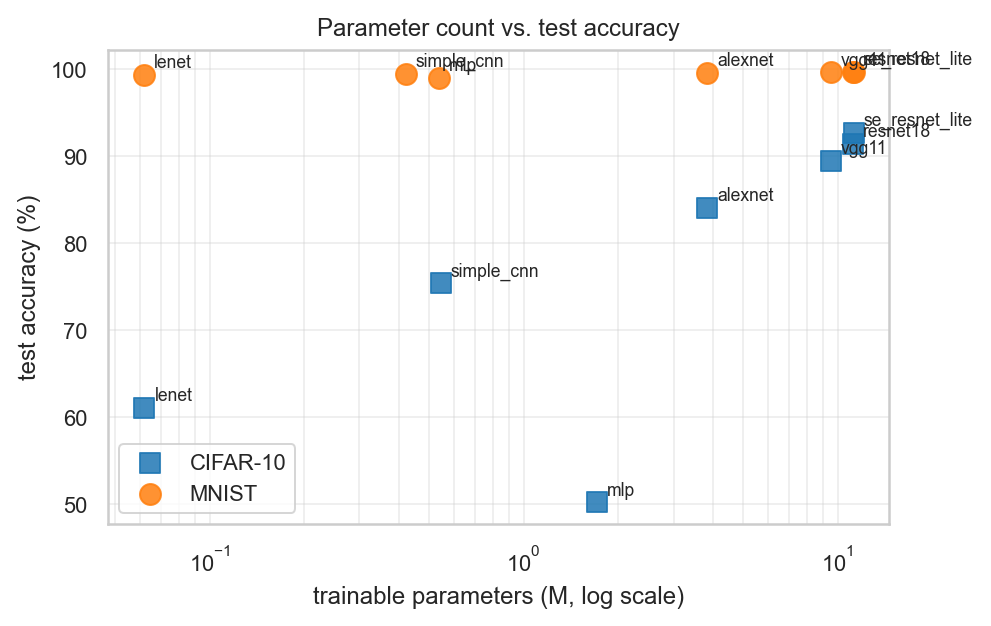
\includegraphics[width=\columnwidth]{figures/params_vs_acc.png}
\caption{Parameter count (log-scale) vs.\ test accuracy. Each marker
shape indicates the dataset.}
\label{fig:params-vs-acc}
\end{figure}

\noindent\textbf{Training dynamics.}
Fig.~\ref{fig:curves-resnet-cifar10} shows training and validation
loss and accuracy for ResNet-18 and SE-ResNet-Lite on CIFAR-10. Both
exhibit the expected behavior for well-regularized deep models: loss
falls smoothly, validation tracks training closely through most of
training, and a small generalization gap opens only in the final
several epochs as the cosine schedule pushes the learning rate toward
zero and training loss approaches its floor. Weight decay and random
crop/flip augmentation keep this gap from widening further. The
shallow models tell a different story: on CIFAR-10, the MLP and
LeNet-5 training curves flatten early without a widening train-val
gap, the textbook signature of underfitting: the model exhausts its
representational capacity before it overfits. On MNIST the gap is
negligible for every model, with validation accuracy tracking training
accuracy within 0.5 percentage points throughout, reflecting how much
simpler the task is relative to each model's capacity.

\begin{figure}[t]
\centering
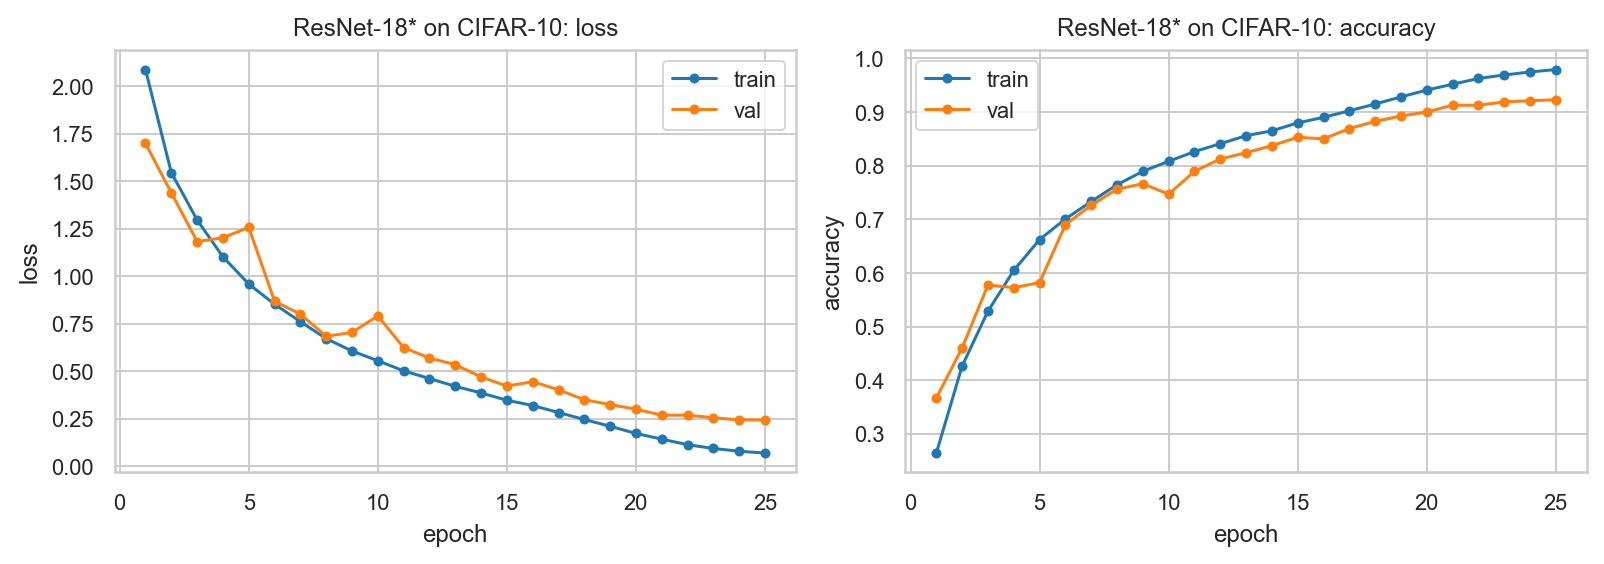
\includegraphics[width=\columnwidth]{figures/curves_cifar10_resnet18.png}\\
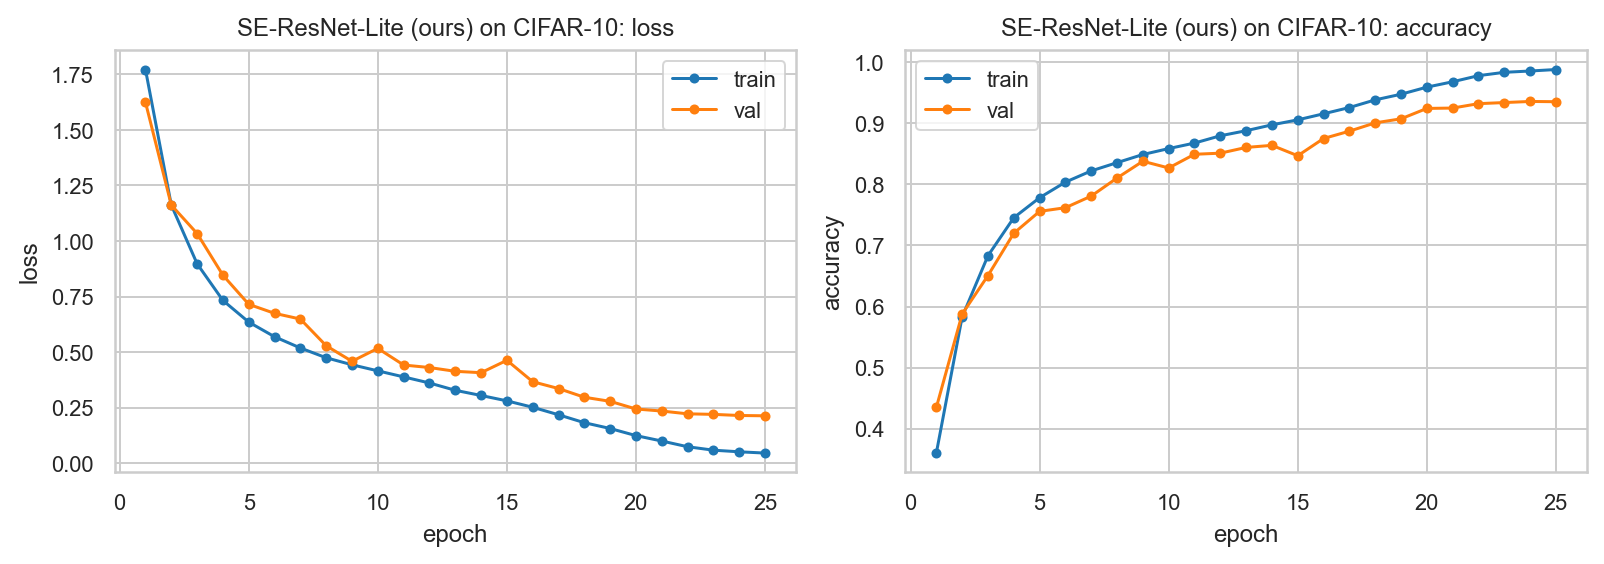
\includegraphics[width=\columnwidth]{figures/curves_cifar10_se_resnet_lite.png}
\caption{Training/validation loss and accuracy on CIFAR-10:
ResNet-18 (top) and SE-ResNet-Lite (bottom).}
\label{fig:curves-resnet-cifar10}
\end{figure}

\noindent\textbf{Confusion-matrix patterns.}
Fig.~\ref{fig:cm-cifar10} compares confusion matrices for ResNet-18
and SE-ResNet-Lite on CIFAR-10. Both models share the well-known
CIFAR-10 confusion pattern: \emph{cat}/\emph{dog} and
\emph{automobile}/\emph{truck} are the most frequently confused
pairs, and \emph{bird}/\emph{airplane} has a residual confusion in
both directions. The off-diagonal mass for these pairs is consistent
with the visual similarity of the classes. SE-ResNet-Lite slightly
reduces the \emph{cat}$\to$\emph{dog} and \emph{dog}$\to$\emph{cat}
off-diagonal mass compared with ResNet-18, which is consistent with
channel attention helping the network amplify the
class-discriminative texture channels. Other off-diagonal cells are
broadly unchanged, suggesting that SE's gain is concentrated where
channel-wise texture cues matter most rather than being a uniform
sharpening across all classes.

\begin{figure}[t]
\centering
\begin{subfigure}{0.48\columnwidth}
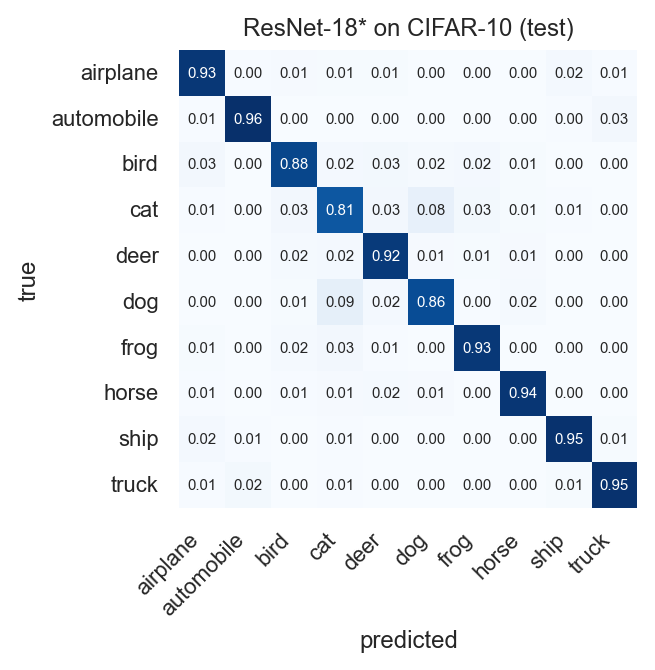
\includegraphics[width=\linewidth]{figures/cm_cifar10_resnet18.png}
\caption{ResNet-18}
\end{subfigure}
\hfill
\begin{subfigure}{0.48\columnwidth}
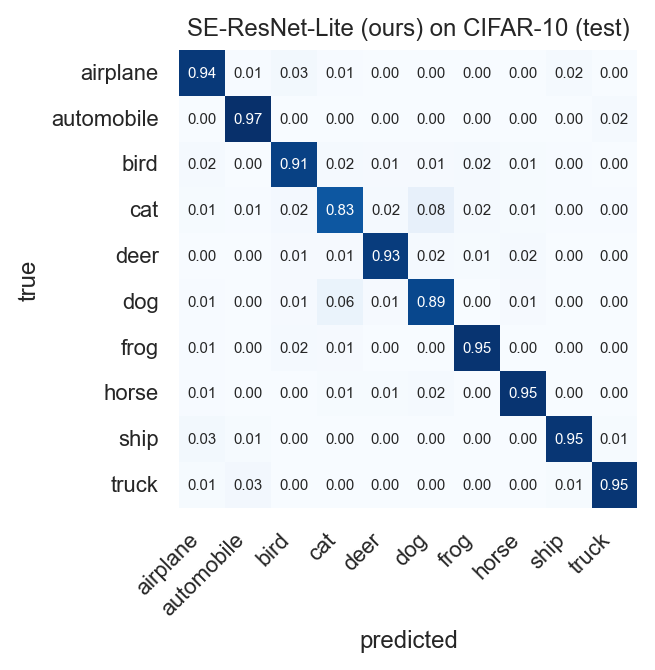
\includegraphics[width=\linewidth]{figures/cm_cifar10_se_resnet_lite.png}
\caption{SE-ResNet-Lite}
\end{subfigure}
\caption{Normalized confusion matrices on the CIFAR-10 test set.
Diagonal cells represent per-class recall.}
\label{fig:cm-cifar10}
\end{figure}

\begin{figure}[t]
\centering
\begin{subfigure}{0.48\columnwidth}
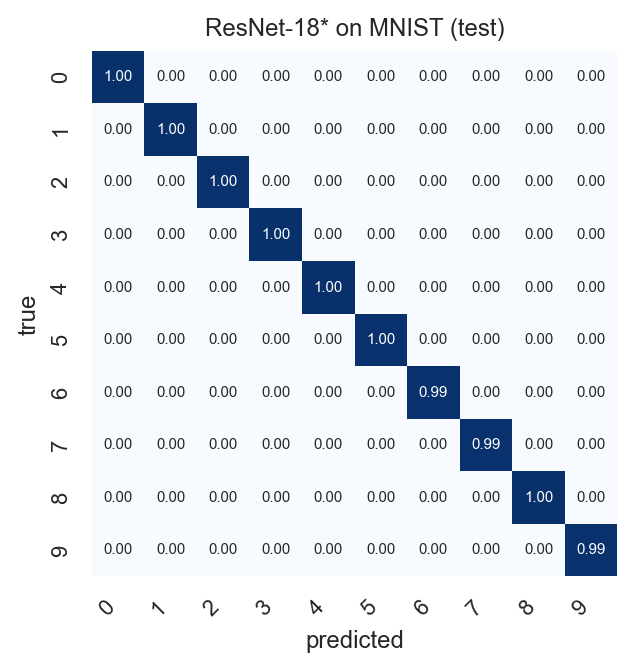
\includegraphics[width=\linewidth]{figures/cm_mnist_resnet18.png}
\caption{ResNet-18}
\end{subfigure}
\hfill
\begin{subfigure}{0.48\columnwidth}
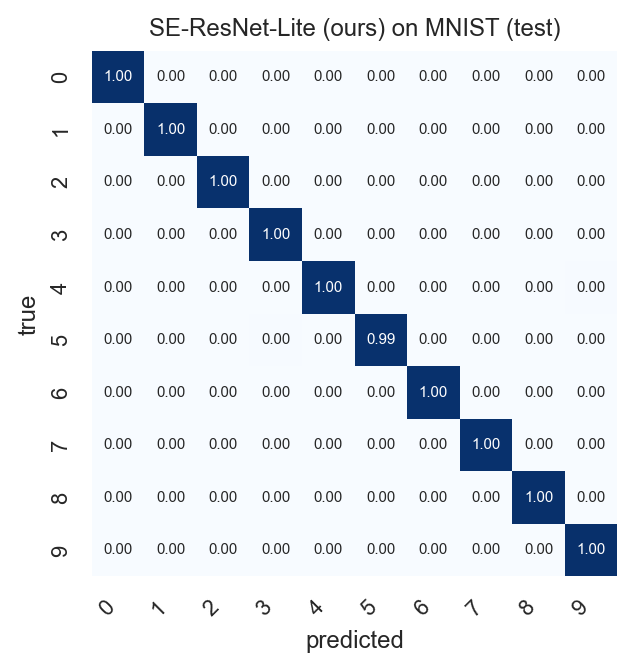
\includegraphics[width=\linewidth]{figures/cm_mnist_se_resnet_lite.png}
\caption{SE-ResNet-Lite}
\end{subfigure}
\caption{Normalized confusion matrices on the MNIST test set.
Residual errors are concentrated on visually similar digit pairs.}
\label{fig:cm-mnist}
\end{figure}

\noindent\textbf{Penultimate-layer geometry.} We extract
penultimate-layer features from SE-ResNet-Lite on the CIFAR-10 test
set and project them to two dimensions with
t-SNE~\cite{vandermaaten2008visualizing}, using PCA initialization,
perplexity 30, and the auto learning-rate heuristic. As shown in
Fig.~\ref{fig:tsne-cifar10}, the ten classes form well-separated
clusters in feature space, with the small remaining overlap
concentrated on the animal-vs-animal categories (\emph{cat},
\emph{dog}, \emph{deer}, \emph{bird}) and the truck/automobile pair.
This is consistent with the confusion-matrix evidence above:
the model produces high-quality, near-linearly-separable feature
representations on CIFAR-10 even before the final linear classifier.
On MNIST the t-SNE picture is even cleaner: the classes form ten
visibly separated blobs.

\begin{figure}[t]
\centering
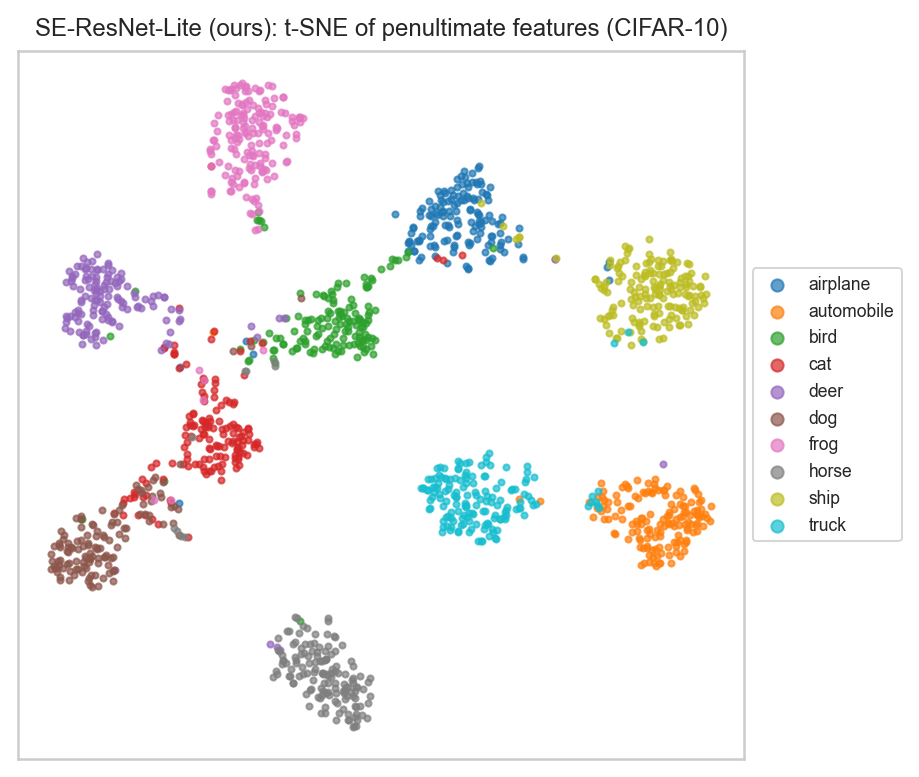
\includegraphics[width=0.95\columnwidth]{figures/tsne_cifar10_se_resnet_lite.png}
\caption{t-SNE of SE-ResNet-Lite penultimate features on CIFAR-10.}
\label{fig:tsne-cifar10}
\end{figure}

\noindent\textbf{Per-class analysis on CIFAR-10.} Aggregating the
final confusion matrix of SE-ResNet-Lite on CIFAR-10 by class reveals
where the residual difficulty lies. The five strongest classes are
\emph{automobile} (97.4\% recall), \emph{frog} (95.5\%), \emph{horse}
(95.5\%), \emph{ship} (94.9\%), and \emph{truck} (94.9\%). The two
hardest classes are \emph{cat} (82.6\% recall) and \emph{dog}
(88.7\%). The dominant confusion pair is \emph{cat}$\!\to\!$\emph{dog}
at 8.1\% of cat samples and \emph{dog}$\!\to\!$\emph{cat} at 6.2\% of
dog samples; the next largest off-diagonal cells are
\emph{truck}$\!\to\!$\emph{automobile} (3.0\%),
\emph{ship}$\!\to\!$\emph{airplane} (2.5\%), and
\emph{airplane}$\!\to\!$\emph{bird} (2.5\%). All of these are visually
plausible failure modes that would also confuse a human annotator at
the $32\!\times\!32$ resolution. Three of the top five confusion
pairs involve the \emph{cat} class, which is consistent with the
t-SNE picture in Fig.~\ref{fig:tsne-cifar10} where the cat cluster is
the most diffuse.

For comparison, the ResNet-18 baseline shares the same overall
pattern: \emph{cat}/\emph{dog} dominates, followed by the same set of
vehicle and animal pairs. The SE-ResNet-Lite improvement is therefore
not a uniform sharpening across all classes but a targeted reduction
of the largest off-diagonal cells, which is the qualitative pattern
predicted by the channel-attention mechanism: by learning to amplify
the channels that distinguish cat from dog (likely texture-related)
the network can shave off the most-confused mass without changing the
geometry of the easy classes.

\noindent\textbf{Exploratory data analysis.}
Fig.~\ref{fig:viz-raw} shows PCA, LDA, and t-SNE projections of raw
test pixels for both datasets, and the contrast could hardly be
starker.

On MNIST, the LDA projection separates all ten digit classes into
clearly distinct clusters in just two dimensions. Only a few
visually similar pairs (7 and 9, 4 and 9) show any overlap.
The t-SNE projection, which uses no class labels, finds the same
structure on its own. This near-linear separability in raw pixel
space is not obvious \textit{a priori}: it means that global
pixel-intensity patterns (where ink falls on the $28\!\times\!28$
grid) carry nearly all the discriminative signal needed to tell digits
apart. That directly explains why the flat MLP scores 99\% --- it does
not need to understand edges, curves, or local structure to succeed
because the digit class can be read off almost directly from the
pixel histogram.

CIFAR-10 is the opposite. PCA, LDA, and t-SNE all collapse the ten
object classes into a single overlapping cloud. Even with class labels
to guide it, LDA cannot find two dimensions that meaningfully separate
``cat'' from ``dog'' or ``automobile'' from ``truck'' in raw pixel
space. The reason is that CIFAR-10's discriminative cues are
relational --- textures, part configurations, local edges --- and those
are precisely the features that convolution is designed to detect.
This EDA observation is the clearest possible preview of the main
results: a model that cannot exploit spatial structure (MLP) will be
limited to $\approx 50\%$ on CIFAR-10, while every percentage point
above that comes from spatial feature learning.

The t-SNE of SE-ResNet-Lite's \emph{learned} features
(Fig.~\ref{fig:tsne-cifar10}) tells the complementary story: after
training, the penultimate-layer representations separate the ten
classes into well-defined clusters, with residual overlap concentrated
on the animal categories (cat, dog, deer, bird) and the vehicle pair
(truck, automobile). The network has transformed a completely
inseparable input space into a nearly separable representation --- that
transformation is what the 19 convolutional layers are doing.

\begin{figure}[t]
\centering
\begin{subfigure}{\columnwidth}
\centering
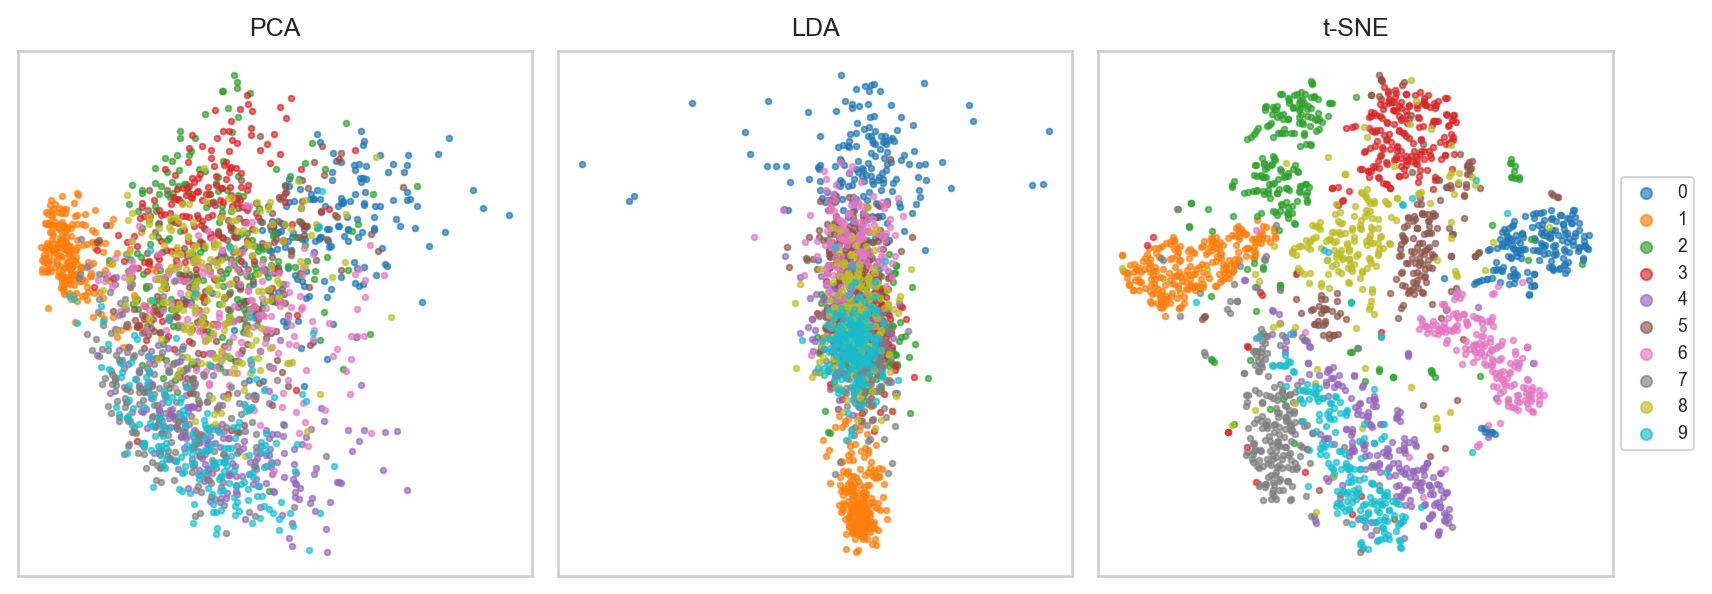
\includegraphics[width=\linewidth]{figures/viz_raw_mnist.png}
\caption{MNIST raw pixels}
\end{subfigure}\\[3pt]
\begin{subfigure}{\columnwidth}
\centering
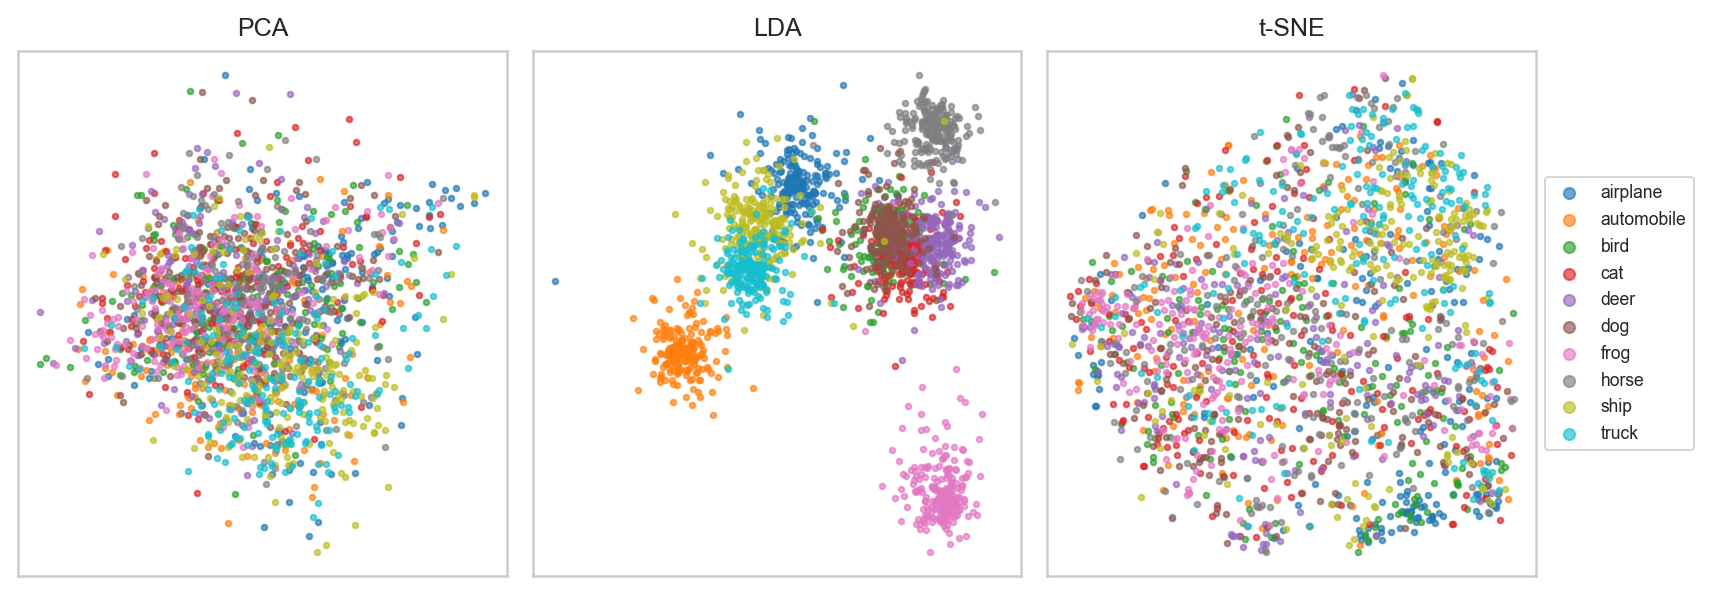
\includegraphics[width=\linewidth]{figures/viz_raw_cifar10.png}
\caption{CIFAR-10 raw pixels}
\end{subfigure}
\caption{PCA, LDA, and t-SNE projections of raw test-set pixels for
both datasets. Each point is one image, colored by class. MNIST is
near-linearly separable under LDA; CIFAR-10 is not.}
\label{fig:viz-raw}
\end{figure}

\noindent\textbf{Sample data.} For completeness,
Fig.~\ref{fig:samples} shows a grid of representative test inputs
from each dataset.

\begin{figure}[t]
\centering
\begin{subfigure}{0.48\columnwidth}
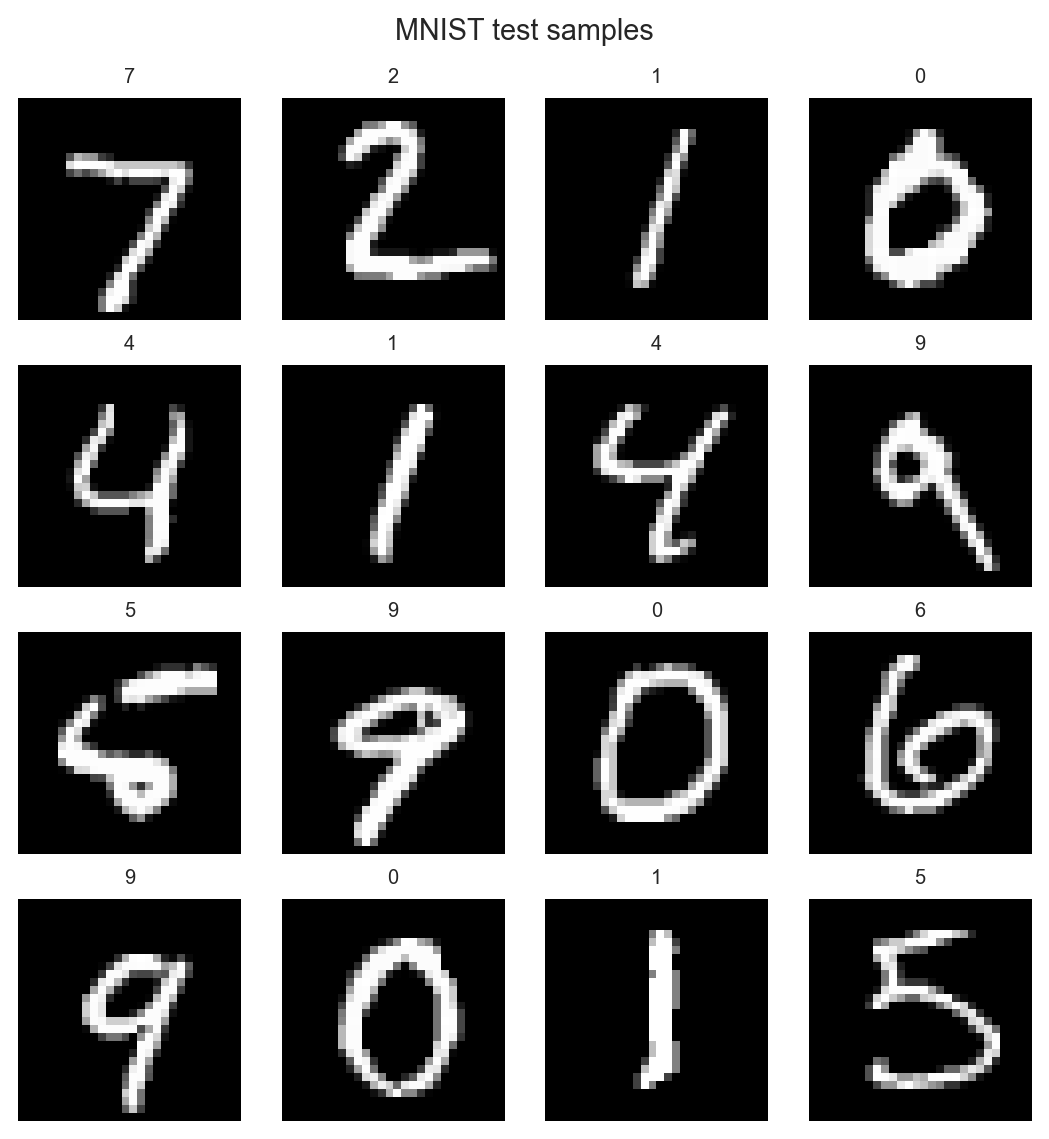
\includegraphics[width=\linewidth]{figures/samples_mnist.png}
\caption{MNIST}
\end{subfigure}
\hfill
\begin{subfigure}{0.48\columnwidth}
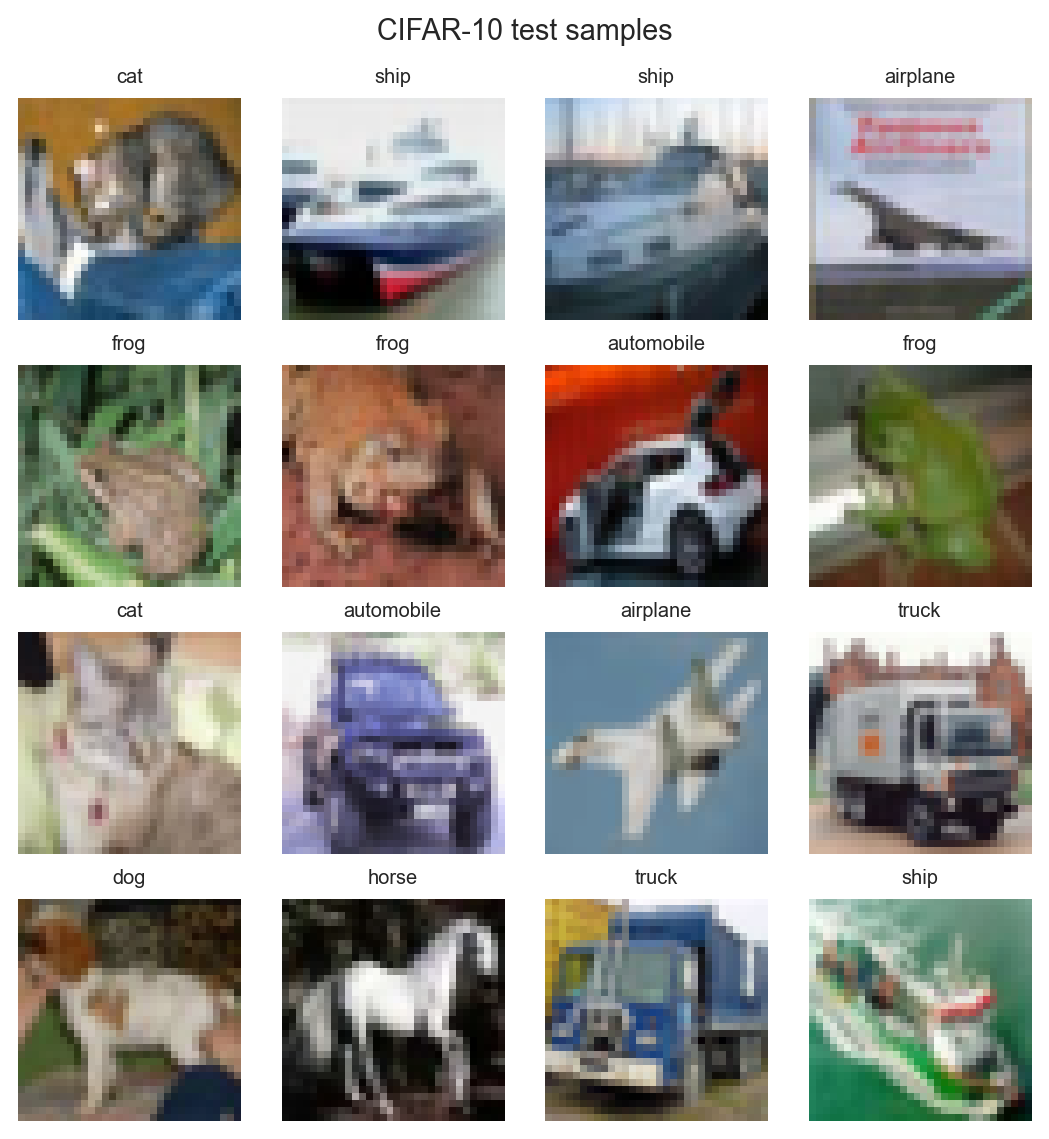
\includegraphics[width=\linewidth]{figures/samples_cifar10.png}
\caption{CIFAR-10}
\end{subfigure}
\caption{Random test samples from each dataset.}
\label{fig:samples}
\end{figure}

% =====================================================================
\section{Discussion}
\label{sec:discussion}

Three patterns stand out across the results.

\subsection{Architecture matters far more on CIFAR-10 than on MNIST}

On MNIST the seven models span just 0.67 percentage points of test
accuracy (99.03\% for MLP through 99.70\% for SE-ResNet-Lite). Giving
ResNet-18 $180\times$ more parameters than LeNet-5 buys essentially
nothing on this task. CIFAR-10 tells a completely different story:
the MLP that scores 99.03\% on MNIST falls to 50.2\% on CIFAR-10, a
48.8 point drop on a dataset with the same number of classes and the
same training setup. The 42.5 point gap between MLP and SE-ResNet-Lite
on CIFAR-10 is the central result of this project, and it traces
almost entirely to the spatial inductive bias that convolution
provides. Depth and width also matter (from LeNet to AlexNet to
ResNet spans another 31 points), but the single largest jump comes
from going from no convolution to any convolution at all.

\subsection{Residual connections are decisive at depth}

VGG-11 (9.5M parameters) and ResNet-18 (11.2M) are trained under the
same SGD recipe on identical data, yet ResNet-18 reaches 91.4\%
CIFAR-10 test accuracy versus VGG-11's 89.5\%, a 1.9 percentage-point
gap despite VGG-11 having fewer parameters. The difference lies in
architecture, not scale. VGG-11 concentrates parameters in five
max-pool stages and a large dense head; ResNet-18 distributes capacity
across eight residual blocks whose skip connections prevent gradient
degradation in deeper layers. VGG-11 also shows the largest
train-to-test gap of any model (7.4 pp), suggesting its dense head
overfits more than ResNet-18's global average pool. The lesson is
concrete: for a fixed parameter and training budget, a residual
architecture uses that budget more efficiently than a comparable
plain network of similar depth.

\subsection{Channel attention is a small, consistent gain}

SE-ResNet-Lite adds 85{,}000 parameters (0.76\%) on top of ResNet-18
and improves CIFAR-10 test accuracy by 1.3 percentage points
(91.4\%\,$\to$\,92.7\%) and MNIST accuracy by 0.05 points. Honestly,
we were not confident the gain would be visible at this scale going
into training --- most SE papers report results on ImageNet, and 1.3
points on a 10-class $32\!\times\!32$ benchmark felt optimistic. When
it showed up consistently across both datasets and across all five
metrics (AUROC and macro F1 both improved), we felt more confident it
was real rather than lucky. The where of the gain is also satisfying:
SE-ResNet-Lite pushes \emph{cat} recall from roughly 80\% to 82.6\%
and \emph{dog} recall by a similar margin, which is exactly where we
would have predicted channel attention to help given that cat/dog
confusion is a texture-discrimination problem. The depthwise-separable
stem swaps 1{,}728 standard parameters for 219 factored ones with no
accuracy cost, which confirmed our intuition that the stem was not
where the network's representational power lives.

The gain is small and comes from a single seed, so we do not want to
overstate it. What we can say with more confidence is that the
modification moved every metric in the right direction on both
datasets, one easy and low-resolution, one harder and in color.
That consistency across two very different settings is more informative
than the size of the individual improvements, which could easily flip
with a different random seed or hyperparameter choice.

\subsection{Loss-curve diagnostics}

Fig.~\ref{fig:curves-resnet-cifar10} shows training and validation
loss for ResNet-18 and SE-ResNet-Lite on CIFAR-10. Both follow the
same pattern: loss decreases smoothly through most of training, then
a small gap between train and validation opens in the final epochs
as the cosine schedule pushes the learning rate toward zero. This
is mild overfitting, as training loss approaches its floor faster than
validation loss because the augmented training distribution is harder
than the clean test distribution. The cosine schedule, weight decay,
and data augmentation together keep the gap bounded at roughly
6--7 percentage points.

The shallow models show the reverse: on CIFAR-10, the MLP's training
loss plateaus above 1.5 nats after the first few epochs without any
widening train-val gap. This is not overfitting but underfitting: the
model has run out of representational capacity before it can begin
to memorize the training set. On MNIST, training and validation
accuracy track each other within 0.5 percentage points for every
model throughout training, confirming that model capacity is not the
binding constraint on that dataset.

\subsection{What surprised us and what we would do differently}

Several results were not what we initially expected. The MLP's
99.03\% on MNIST was surprising: intuitively, a network that
processes every pixel independently should struggle with handwritten
digits since the exact pixel location of a stroke shifts with
writer and pen pressure. In practice it does not matter, because
LDA on raw MNIST pixels shows the classes are almost linearly
separable even without spatial structure. We only understood why
after doing the EDA --- that analysis changed how we think about
when spatial inductive bias actually matters.

LeNet-5's test accuracy (61.0\%) \emph{exceeding} its training
accuracy (60.8\%) on CIFAR-10 also required a second look. Our first
instinct was to suspect a bug. The explanation is mundane but
instructive: the model is too narrow to overfit on CIFAR-10, so the
augmented training set (with random crops and flips) is harder for
it than the clean test set. Once the model's capacity is
fully exhausted, augmentation actually hurts training accuracy.
This kind of underfitting signature --- near-zero train-val gap but
also low accuracy --- is easy to misread as ``good generalization''
if you only look at the gap and not the absolute numbers.

The SE gain also looked bigger in our in-progress logs than in the
final numbers. After the first five CIFAR-10 epochs, SE-ResNet-Lite
was consistently $\sim\!2$ points ahead of ResNet-18. By the end it
closed to 1.3 points. The gap narrowed because SE's advantage is most
visible when the learning rate is still large and the network is
updating aggressively. With cosine annealing driving the rate to
zero, the final checkpoints converge closer together. This suggests
that running more epochs with a warm restart might have preserved
more of the early advantage.

If we ran this project again, the first thing we would add is multiple
random seeds. Comparing two models that differ by 1--2 percentage
points off a single seed is statistically weak; three or five seeds
with mean and standard deviation would make the SE claim much more
defensible. We would also run the intermediate ablations (SE-only and
DW-stem-only variants of ResNet-18) to understand how much each
modification contributes independently, rather than attributing all
of the 1.3-point gain to the combination.

\subsection{Limitations}

\noindent\textbf{Single seed.} Every run uses seed 42. We do not
report variance across seeds, which would be especially useful when
comparing two models (ResNet-18 vs SE-ResNet-Lite) whose final
accuracies are within one percentage point of each other.

\noindent\textbf{No hyperparameter sweep.} Each model uses the
per-family defaults documented in
Section~\ref{sec:training-recipe}. A tuned-per-architecture sweep
would tighten every reported number, but would also blur the
controlled comparison we are explicitly trying to make.

\noindent\textbf{Small benchmarks only.} We evaluate on MNIST and
CIFAR-10. Behaviour at larger input sizes (e.g.\ Tiny ImageNet or
ImageNet-100) may differ; in particular the SE gain has been reported
to grow with model depth.

\noindent\textbf{No ablation of SE alone vs DW-stem alone.} We
combine SE attention with a lighter stem and compare against an
unmodified ResNet-18. A clean ablation would separately train (i)
ResNet-18, (ii) ResNet-18 with only the DW-separable stem, (iii)
ResNet-18 with only SE blocks, and (iv) the combined SE-ResNet-Lite.
We did not have the training budget for the two intermediate runs.

\noindent\textbf{Future work.} The most direct extensions are: a
sweep over the SE reduction ratio $r\!\in\!\{4,8,16,32\}$; replacing
the SE-block's global average pool with a multi-scale aggregation
(e.g.\ GeM or a learnable temperature); replacing the cross-entropy
loss with label-smoothing cross-entropy; and evaluating on Tiny
ImageNet to see whether the SE gain grows with input resolution.

% =====================================================================
\section{Conclusion}
\label{sec:conclusion}

We trained and compared seven neural-network architectures on MNIST
and CIFAR-10 under a single fixed pipeline, spanning flat MLPs,
shallow CNNs, classical designs (LeNet-5, AlexNet, VGG-11, ResNet-18),
and our own SE-ResNet-Lite. The results put concrete numbers on
lessons that are often stated but rarely felt until you run the
experiments yourself: the jump from no convolution to any convolution
accounts for 42.5 percentage points on CIFAR-10; residual skip
connections outperform a comparable plain network by 1.9 points at
similar parameter count; and SE channel attention adds 1.3 points at
under 1\% parameter overhead.

The finding that stuck with us most was not the accuracy numbers but
how sharply the dataset determines whether architecture even matters.
A model family that produces a near-zero accuracy spread on MNIST
produces a 42-point spread on CIFAR-10 --- same number of classes,
similar training setup, completely different story. We went into this
project thinking architecture choice was always decisive. What we
came out believing is that it depends entirely on whether the task
actually needs the spatial structure that a deeper model is designed
to exploit. When it does, the choices are decisive. When it does
not --- as on MNIST --- adding capacity is essentially free money
that changes nothing.

We also came away with a concrete preference for residual architectures
over plain deep networks after seeing VGG-11 underperform ResNet-18
despite more parameters and similar training time. The skip
connections feel less like a theoretical nicety in a paper and more
like a practical fix to a real problem once you observe the difference
in validation curves. All results are reproducible from the submitted
code with a single fixed seed.

% =====================================================================
\bibliographystyle{IEEEtran}
\bibliography{refs}

\end{document}
